


% Bounded identity
\begin{frame}{\tciii{} Signed distances}

\begin{columns}
\begin{column}{0.45\linewidth}
\begin{block}{Bounded identity function}
\begin{equation}
\alpha: \begin{cases}
& \text{ if } x \geq 1: \alpha(x) = 1\\ 
& \text{ if } x \leq -1: \alpha(x) = -1\\ 
& \text{ else: }  \alpha(x) = x
\end{cases}
\end{equation}
\end{block}
\end{column}

\begin{column}{0.45\linewidth}
\begin{figure}
\centering
\includegraphics[width=.9\linewidth]{images/GENE/images/bounded.png}
\end{figure}
\end{column}
\end{columns}

\end{frame}


% Final functions
\begin{frame}{\tciii{} Distance functions}

\begin{columns}
\begin{column}{0.60\linewidth}
\begin{block}{pL2-GENE}
\begin{equation}
\alpha \left  ( \prod_{k=1}^D n_1^k - n_2^k \right ) \sqrt{\sum_{j=1}^D \left( n_1^j - n_2^j \right)^2 }
\end{equation}
\end{block}
\end{column}

\begin{column}{0.35\linewidth}
\begin{figure}
\centering
\includegraphics[width=\linewidth]{images/GENE/images/distance_pL2.png}
\end{figure}
\end{column}
\end{columns}

\begin{columns}
\begin{column}{0.60\linewidth}
\begin{block}{tag-GENE}
\begin{equation}
\sum_{j=2}^D \alpha(n_1^j - n_2^1) e^{-|n_1^j - n_2^1|}
\end{equation}
\end{block}
\end{column}

\begin{column}{0.35\linewidth}
\begin{figure}
\centering
\includegraphics[width=\linewidth]{images/GENE/images/distance_tag.png}
\end{figure}
\end{column}
\end{columns}

\end{frame}


\begin{frame}{\tcv{} The \lucie{} selection procedure}%
    \vspace{1em}
    \onslide<2->{%
        \textbf{Objective:} identify the {\color<2>{cyan}\textbf{best $\mu$}} individuals with as {\color<2>{magenta}\textbf{few evaluations}} as possible.
    }
    \vspace{1em}
    \begin{figure}
        \def\xmax{10}%
        \def\ymax{5}%
        \def\dx{1.3}%
        \def\hicol{magenta}%
        \def\locol{cyan}%
        \def\elcol{green!60!black}%
        \begin{tikzpicture}[%
                ball/.style={circle,inner sep=0,outer sep=0,minimum width=2mm}
            ]%
            % axis
            \onslide<3->{%
                \draw [stealth-stealth,thick] (0,\ymax) node (yaxis) [above] {} |- (\xmax,0) node (xaxis) [right] {};
                \node[rotate=90] at (-0.4,\ymax-0.7) {\textsc{Fitness}};
                \node[] at (\xmax-1.1,-0.4) {\textsc{Individuals}};
            }
            % individuals
            \onslide<4->{%
                \foreach \x in {1,2,3,4,5}{%
                    \node[ball,fill=black,opacity=1.0] at (\x*\dx,0){};
                }
            }
            \onslide<5>{%
                % mean
                \node[] (i1mean) at (1*\dx,2.5) {};
                \node[red] (mean) at (5,4) {\textbf{Empirical mean:} $\hat{f} = \frac{1}{u} \sumc{k=1}{u} y_k$};
                \draw[red,-stealth] (mean.west) to[out=180,in=0] (i1mean.east);
                % ci
                \node[] (i1ci) at (0.1+1*\dx,2.0) {};
                \node[red] (ci) at (5,0.5) {\textbf{Confidence interval:} $\beta(u,t)$};
                \draw[red,-stealth] (ci.west) to[out=180,in=0] (i1ci.east);
                \roundbracket{0.2+1*\dx}{2.0}{0.45}{red}{0.08}{}{90}% x y width color sidesize thickness rotate
            }
            % t=1 fitnesses
            \onslide<5-7>{%
                \only<5>{%
                    \cifit{1*\dx}{2.5}{1}{black} % x y beta color
                    \cifit{2*\dx}{2.4}{1}{black}
                    \cifit{3*\dx}{2.3}{1}{black}
                    \cifit{4*\dx}{2.3}{1}{black}
                    \cifit{5*\dx}{2.1}{1}{black}
                }
                \only<6->{%
                    \cifit{1*\dx}{2.5}{1}{\hicol} % x y beta color
                    \cifit{2*\dx}{2.4}{1}{\hicol}
                    \cifit{3*\dx}{2.3}{1}{\locol}
                    \cifit{4*\dx}{2.3}{1}{\locol}
                    \cifit{5*\dx}{2.1}{1}{\locol}
                }
            }
            % high low sets
            \onslide<6-8>{%
                \node[] at (1.5*\dx,4) {\color{\hicol}\textsc{High}};
                \node[] at (4.0*\dx,4) {\color{\locol}\textsc{Low}};
                \roundbracket{1.5*\dx}{3.8}{0.6*\dx}{\hicol}{0.1}{}{180}
                \roundbracket{4.0*\dx}{3.8}{1.1*\dx}{\locol}{0.1}{}{180}
            }
            % sampling candidates 1
            \onslide<7>{%
                \node[draw, rounded corners=0.1cm] (sc) at (2.5*\dx,-1) {Sampling candidates};
                \draw[-stealth] (sc.north) to[out=90,in=-90] (2*\dx,-0.1);
                \draw[-stealth] (sc.north) to[out=90,in=-90] (3*\dx,-0.1);
                \node[ball,draw,dashed,thick,minimum width=0.5cm] at (2*\dx,1.4) {};
                \node[ball,draw,dashed,thick,minimum width=0.5cm] at (3*\dx,3.3) {};
            }
            % t=2 fitnesses
            \onslide<8>{%
                \cifit{1*\dx}{2.5}{1}{\hicol} % x y beta color
                \cifit{2*\dx}{2.4}{0.7}{\hicol}
                \cifit{3*\dx}{2.3}{0.7}{\locol}
                \cifit{4*\dx}{2.3}{1}{\locol}
                \cifit{5*\dx}{2.1}{1}{\locol}
            }
            % sampling candidates 2
            \onslide<8>{%
                \node[draw, rounded corners=0.1cm] (sc) at (2.5*\dx,-1) {Sampling candidates};
                \draw[-stealth] (sc.north) to[out=90,in=-90] (1*\dx,-0.1);
                \draw[-stealth] (sc.north) to[out=90,in=-90] (4*\dx,-0.1);
                \node[ball,draw,dashed,thick,minimum width=0.5cm] at (1*\dx,1.5) {};
                \node[ball,draw,dashed,thick,minimum width=0.5cm] at (4*\dx,3.3) {};
            }
            % t=3 fitnesses + stop
            \onslide<9->{%
                % stop
                \draw[thick, dashed] (2*\dx,2.3) -- (6*\dx,2.3);
                \draw[thick, dashed] (3*\dx,2.5) -- (6*\dx,2.5);
                \draw[thick] (6*\dx,2.3-0.5) -- (6*\dx,2.5+0.5);
                \draw[thick,-stealth] (6*\dx,2.3-0.5) -- (6*\dx,2.3);
                \draw[thick,-stealth] (6*\dx,2.5+0.5) -- (6*\dx,2.5);
                \node[] at (6.5*\dx,2.4) {$\leq \epsilon$};
                \node[] at (6.5*\dx,3.4) {Stopping Criterion:};
                % sets
                \node[] at (1.5*\dx,4.9) {\color{\hicol}\textsc{High}};
                \node[] at (4.0*\dx,4.9) {\color{\locol}\textsc{Low}};
                \roundbracket{1.5*\dx}{4.7}{0.6*\dx}{\hicol}{0.1}{}{180}
                \roundbracket{4.0*\dx}{4.7}{1.1*\dx}{\locol}{0.1}{}{180}
                % fit
                \cifit{1*\dx}{3.5}{1}{\hicol} % x y beta color
                \cifit{2*\dx}{2.8}{0.5}{\hicol}
                \cifit{3*\dx}{1.8}{0.7}{\locol}
                \cifit{4*\dx}{1.5}{0.5}{\locol}
                \cifit{5*\dx}{1.2}{0.9}{\locol}
                % elite
                \node[ball,fill=\elcol] at (1*\dx,0){};
                \node[ball,fill=\elcol] at (2*\dx,0){};
                \node[] at (1.5*\dx,-0.5) {\color{\elcol}\textsc{Elite}};
                \roundbracket{1.5*\dx}{-0.3}{0.6*\dx}{\elcol}{0.1}{}{0}
            }
        \end{tikzpicture}%
    \end{figure}
\end{frame}


\begin{frame}{\tcv{} Classic Control}%
        \def\figwidth{0.16\linewidth}%
        \def\yleg{Fitness}%
        \begin{textblock*}{2cm}(0cm,0.7cm) % {block width} (coords)
            $\%$noise
        \end{textblock*}
        \begin{table}%[!t]
            \centering
            \begin{tabular}{ccccccc}
                && $0\%$ & $200\%$ & $400\%$ & $600\%$ & $800\%$ \\
                \raisebox{3\normalbaselineskip}[0pt][0pt]{\rotatebox[origin=c]{90}{\cartpole}} &
                \raisebox{3\normalbaselineskip}[1cm][0cm]{\rotatebox[origin=c]{90}{\vspace{1cm}\yleg}}&
                \includegraphics[width=\figwidth]{images/LUCIE/cartpole/boxplot_cartpole_0.png} &
                \includegraphics[width=\figwidth]{images/LUCIE/cartpole/boxplot_cartpole_200.png} &
                \includegraphics[width=\figwidth]{images/LUCIE/cartpole/boxplot_cartpole_400.png} &
                \includegraphics[width=\figwidth]{images/LUCIE/cartpole/boxplot_cartpole_600.png} &
                \includegraphics[width=\figwidth]{images/LUCIE/cartpole/boxplot_cartpole_800.png}\\
            \end{tabular}
%				\caption{Final validation fitness for \cartpole{} neuroevolution under posterior uniform noise.}
%				\label{table:cartpole-uniform-eval-validation}
        \end{table}

        \vspace{-1em}

        \def\figwidth{0.16\linewidth}
        \def\yleg{Fitness}
        \begin{table}[]
            \centering
            \begin{tabular}{ccccccc}
%					&& 0\% & 200\% & 400\% & 600\% & 800\% \\
                \raisebox{3.5\normalbaselineskip}[0pt][0pt]{\rotatebox[origin=c]{90}{\acrobot{}}} &
                \raisebox{3.5\normalbaselineskip}[1cm][0cm]{\rotatebox[origin=c]{90}{\vspace{1cm}\yleg}}&
                \includegraphics[width=\figwidth]{images/LUCIE/acrobot/boxplot_acrobot_0_u.png} &
                \includegraphics[width=\figwidth]{images/LUCIE/acrobot/boxplot_acrobot_200_u.png} &
                \includegraphics[width=\figwidth]{images/LUCIE/acrobot/boxplot_acrobot_400_u.png} &
                \includegraphics[width=\figwidth]{images/LUCIE/acrobot/boxplot_acrobot_600_u.png} &
                \includegraphics[width=\figwidth]{images/LUCIE/acrobot/boxplot_acrobot_800_u.png}\\
            \end{tabular}
%				\caption{Final validation fitness for Acrobot neuroevolution under posterior uniform noise.}
%				\label{table:acrobot-uniform-eval-validation}
        \end{table}

\end{frame}

